% Curation with a person in the loop: the model suggests, the curator decides.
% ---------------------------------------------------------------------------
% style.tex --- shared preamble for every figure in book/figures/tikz/
%
% One style for all figures: Latin Modern, thin black lines, a light grey
% fill, and one accent colour used only to mark what is untrusted or wrong.
% Build with scripts/build_figures.sh; see book/figures/README.md.
% ---------------------------------------------------------------------------
\documentclass[tikz,border=6pt]{standalone}
\usepackage[T1]{fontenc}
\usepackage{lmodern}
\usetikzlibrary{arrows.meta,positioning,shapes.geometric,calc,fit,backgrounds}

\hyphenpenalty=10000   % short lines in boxes: ragged, never hyphenated

\definecolor{lightgrey}{gray}{0.92}
\definecolor{accent}{HTML}{9B2D20}

\tikzset{
  every picture/.style={
    line width=0.6pt,
    font=\small,
    >={Stealth[length=5pt,width=4pt]},
    node distance=14pt and 24pt,
  },
  % shapes
  box/.style={draw, rectangle, inner xsep=8pt, inner ysep=5pt,
              minimum height=22pt, align=center},
  grey/.style={box, fill=lightgrey},
  rounded/.style={box, rounded corners=9pt},
  decision/.style={draw, diamond, aspect=2.4, inner sep=1.5pt, align=center},
  group/.style={draw, dashed, rounded corners=5pt, inner sep=7pt},
  % text
  tag/.style={font=\footnotesize, align=center, inner sep=2pt},
  note/.style={font=\footnotesize\itshape, align=center, inner sep=2pt},
  code/.style={font=\small\ttfamily},
  codetag/.style={font=\footnotesize\ttfamily, align=center, inner sep=2pt},
  title/.style={font=\small\scshape, align=center, inner sep=2pt},
  % lines
  arrow/.style={->},
  back/.style={->, dashed},
  thin/.style={line width=0.4pt, gray},
  % the one accent, for what is untrusted, wrong or missing
  bad/.style={accent},
  badbox/.style={box, draw=accent, text=accent},
}

\begin{document}
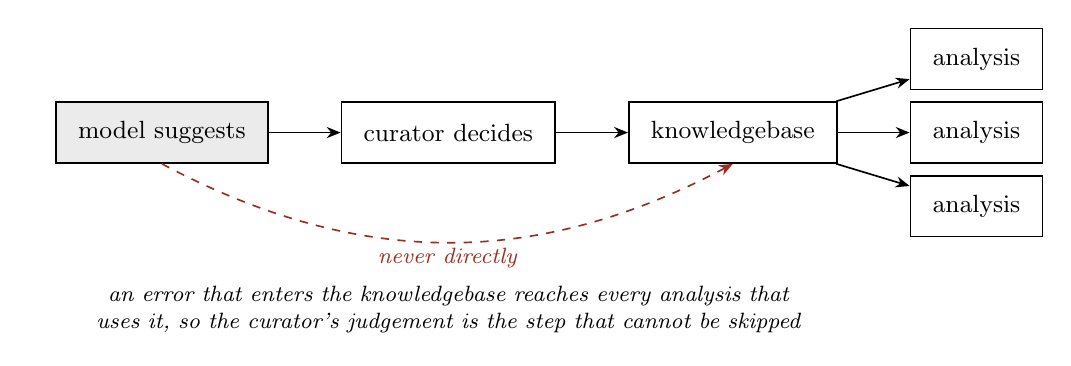
\begin{tikzpicture}[node distance=10pt and 26pt]
  \node[grey] (m) {model suggests};
  \node[box, right=of m] (c) {curator decides};
  \node[box, right=of c] (kb) {knowledgebase};
  \node[box, above right=4pt and 26pt of kb] (a1) {analysis};
  \node[box, right=of kb] (a2) {analysis};
  \node[box, below right=4pt and 26pt of kb] (a3) {analysis};
  \draw[->] (m) -- (c);
  \draw[->] (c) -- (kb);
  \draw[->] (kb) -- (a1);
  \draw[->] (kb) -- (a2);
  \draw[->] (kb) -- (a3);
  \draw[back, bad] (m.south) to[bend right=28] node[note, below, text=accent] {never directly} (kb.south);
  \node[note, below=42pt of c, text width=300pt]
    {an error that enters the knowledgebase reaches every analysis that uses it,
     so the curator's judgement is the step that cannot be skipped};
\end{tikzpicture}
\end{document}
